\chapter{INTEREST AND DEBT}
\begin{chapquote}{Aaron Swartz}
``Be curious. Read widely. Try new things. What people call intelligence just boils down to curiosity.''
\end{chapquote}

\section{Forms of interest}
\subsection{Compound and simple interest}
If you deposit a total sum of money $S$ to a bank with a compound annual interest of $r$\footnote{I'll always assume risk-free interest rates, if not specified.} (e.g., $r=0.1=10\%$) and you wait $n$ years, then your new total sum will be:

\begin{equation}\label{eq:annual_compound_interest}
S' = S(1+r)^n .
\end{equation}

In case of simple annual interest, after $T$ years you would have:

\begin{equation}\label{eq:annual_simple_interest}
S' = S\big(1+rT\big) .
\end{equation}

From equation~\ref{eq:annual_compound_interest} we can compute the number of years $n$ needed to increase our initial sum $S$ of a factor $\beta$:

\begin{equation}\label{eq:time_to_double}
n = \dfrac{\ln{\beta}}{\ln{1+r}}.
\end{equation}

\subsection{The rule of 72}
An approximation to quickly evaluate the time needed to double our money is "the rule of 72". Assume again we have a compound annual interest $r$, then we have to wait $\dfrac{72}{100r}$ years. If the compound interest is a monthly interest, then it would be $\dfrac{72}{100r}$ months. Simple example: with a compound annual interest of $r=9\%$ we should wait 8 years.

\subsection{Continuous compounding interest}
If I lend you a sum $S$ for one year with an interest rate $r$, then at the end of the year you owe me $S'=S(r+1)$. But let's suppose that you may be able to give me the money back in a half a year. In this case, I'd reasonably half the interest at $r'=r/2$, hence you'll give me $S'=S(r'+1)$, but if you miss the payment, then I'll lend you $S'$ at the same interest for another half year, so you'll pay me $S''=S(r'+1)^2$.
If you want to try to set a monthly deadline instead of a semestral one, than it'd be:

\begin{equation}\label{eq:tmp}
S'=S\bigg(1+\dfrac{r}{12}\bigg)^{12}.
\end{equation}

You could also consider days or hours instead of months. If $r=1$ and the interval is infinitesimal, you'll get $S'=eS$, where $e$ is the Euler's number. More generally, if I lend you money for $T$ years and we compound $n$ times per year then it'd be:

\begin{equation}\label{eq:tmp_general}
S'=S\bigg(1+\dfrac{r}{n}\bigg)^{nT}.
\end{equation}

Using the previous limit to get $e$ we can compute the formula for continuous compounding interest:

\begin{equation}\label{eq:continuous_compounding_interest}
S'=Se^{nT}.
\end{equation}

\section{Time value of money}
\subsection{Discounting}
If I have now an amount $S$ of money, then $S$ is the present value. If I have the option of a compound annual interest rate $r$, then the future value $S'$ in $n$ years would be the one obtained in equation~\ref{eq:annual_compound_interest}. So if I'm told that someone is willing to give me $S'$ in $n$ years, I can compute the present value $S$ simply as:

\begin{equation}\label{eq:annual_discount_interest}
S = \dfrac{S'}{(1+r)^n} .
\end{equation}

This is known as discounting. If the interest rate decreases the present value of $S'$ will increase. Discount rates can change depending on the time the money is lent for. The longer the period, the higher the rate.

The annual percentage rate ($APR$) can be obtained from compounding the daily percentage rate ($DPR$):

\begin{equation}\label{eq:APR}
APR = 365 \cdot DPR .
\end{equation}

Alternatively, the money $S'$ owed at day $d$ would be:

\begin{equation}\label{eq:DPR}
S' = S (1+DPR)^d.
\end{equation}

Due to decimal number precision, the result of equation~\ref{eq:DPR}, which is the effective $APR$ may differ from $S\cdot APR$.

\section{Additional notes}

\subsection{Risk-free and risk premium}
Think of an interest rate as the cost of money, which just like the cost of production, labor, and other expenses is a factor of a company's profitability.

The fundamental cost of money to an investor is the Treasury note rate, whose return is guaranteed by the "full faith and credit" of the U.S. government. According to financial theory, a stock's value proposition starts there: stocks are risky assets, even riskier than bonds because bondholders are paid their capital before stockholders in the event of bankruptcy. Therefore, investors require a higher return for taking on extra risk by investing in stocks instead of Treasury notes, which are guaranteed to pay a certain return.

The extra return that investors can theoretically expect from stocks is referred to as the "risk premium." Historically, the risk premium runs at around five percent. This means that if the risk-free rate (the Treasury note rate) is four percent, then investors would demand a return of nine percent from a stock. Therefore, the total return on a stock is the sum of two parts: the risk-free rate and the risk premium.

\subsection{Required rate of return}
The required rate of return is the minimum return an investor expects to achieve by investing in a project. An investor typically sets the required rate of return by adding a risk premium to the interest percentage that could be gained by investing excess funds in a risk-free investment.

There is an inverse relationship between required return and the price investors assign to a stock. Why? Let's say people in the market are looking for a way to make \$10 from investing and they all decide to buy stock A because it has a price of \$100 and will give exactly a ROC of 10\% after one year. Let's say that after one year people want to invest again, but this time the company is expected to perform better and have a ROC of 20\%. If people are still looking for an income of \$10, they will buy stock A for \$50. In this case, higher return means lower price (with fixed income). If instead there is more money to be invested and more people is investing, they will be willing to pay higher prices for the same income, which means lower returns. 

If interest rates are high, the cost of money will be high. This means that for a company to borrow money will be more difficult and it will have to work harder and generate higher returns. High interest rates normally prevent people from buying things and companies from investing in growth opportunities. As a result, sales and profits drop, as do share prices.

% \begin{figure}
%     \centering
%     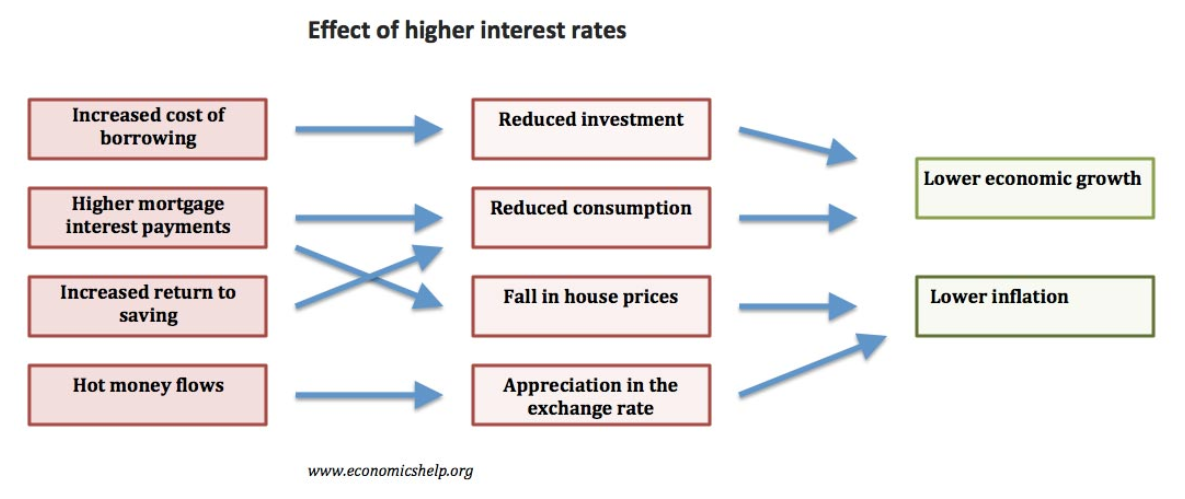
\includegraphics{images/high_rates.png}
%     \caption{}
%     \label{fig:my_label}
% \end{figure}
